\documentclass[portrait,final]{fermiposter}

% Folder(s) where LaTex is supposed to search for figures.
\graphicspath{{figures/}}

% Title, authors and affiliations.
\title{Cosmic-Ray Nuclei in the Fermi-LAT}
\author[1,2]{David Green}
\author[2]{T. J. Brandt}
\author[2]{E. Hays}
\affil[1]{University of Maryland}
 \affil[2]{NASA-GSFC}
\collaboration{Fermi Large Area Telescope}

\begin{document}

\begin{poster}
  { % Poster Options---change stuff at your leisure.
    grid            = no             , % Visualize a debug grid.
    headerheight    = 0.1\textheight, % The height of the title/author block.
    titlefont       = \bf\Huge       , % Font for the title.
    authorfont      = \large         , % Font for the authors/affiliations.
    abstractfont    = \small         , % Font for the abstract box.
    headerfont      = \bf\Large      , % Font for the box headers.
    textfont        = \small    , % Font for the body text.
    textmargin      = 0.5em          , % Left/right margins for the body text.
    textcolor       = blue           , % Default text color.
    twocolsabstract = no             , % Use two columns for the abstract.
    linewidth       = 2pt              % Width of the lines.
  }
  { % Fermi logo.
    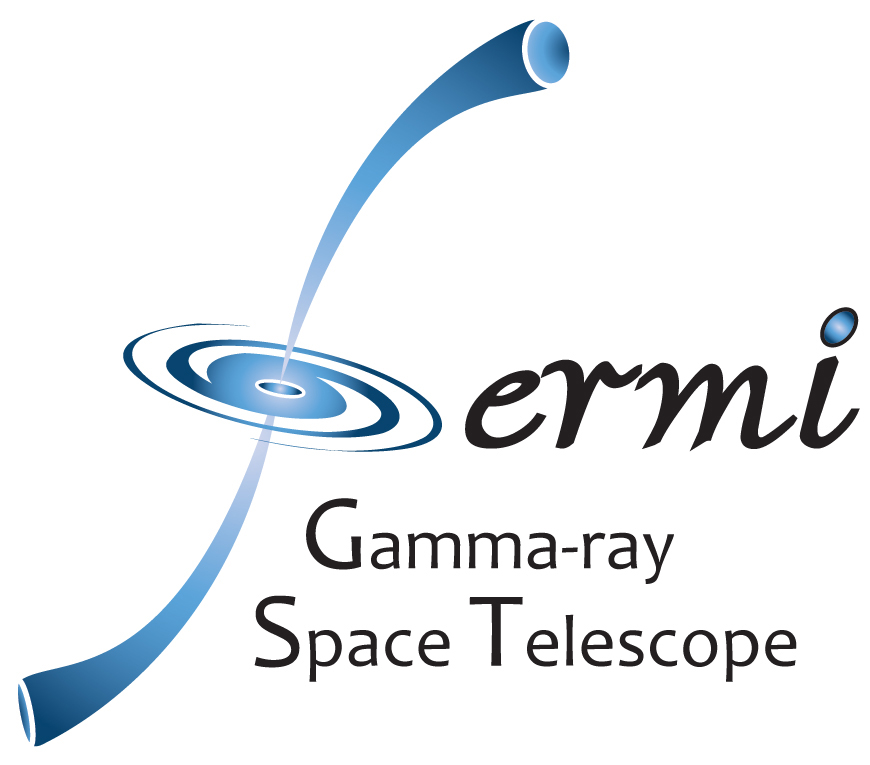
\includegraphics[width=0.15\textwidth]{fermi_logo_large}
  }
  { % Your own logo.
    \includegraphics[width=0.15\textwidth]{NASA-logo}
    %    
\includegraphics[width=0.15\textwidth]{umd-logo}
    
%        \begin{minipage}[t]{0.15\textwidth}
%              \vspace{0pt} % Yes: you need this one...
%    \includegraphics[width=0.075\textwidth]{NASA-logo}
%    \includegraphics[width=0.075\textwidth]{UMD-logo}
%        \end{minipage}

  }
 
 
  \abstract{}{    
The Anti-Coincidence Detector (ACD) of the Fermi Large Area Telescope (LAT) serves to identify charged particles which cross the LAT at a rate orders of magnitude higher than that of the $\gamma$-ray signal. We have developed a method that uses cosmic-ray nuclei, Z > 3, as a calibration source to improve signal uniformity, gain linearity, and charge resolution of light deposit measurement in the ACD at high light levels. In addition we present a preliminary study to measure cosmic ray energy via the calorimeter (CAL).  We present the results of our method and demonstrate improved signal uniformity and charge resolution for cosmic-ray nuclei in the ACD.
  }


  % Your first box. If you specify the height, that's relative to the
  % poster height (0.3 is 30% of the poster). If you don't the box will
  % adapt itself to the content.
  \headerbox{Goals and Motivation}{name=goals,column=0,span=3,
    below=abstract,height=0.22}{

    \begin{minipage}[t]{0.5\textwidth}
      \vspace{0pt} % Yes: you need this one...

\begin{itemize}
\item \textbf{Goal}: Study energy dependence of the Boron to Carbon ratio using the LAT
\item \emph{Fermi} could measure the Boron to Carbon at energies $\geq$ 1 TeV/n
\begin{itemize}
\item Less atmospheric contamination when compared to balloon-borne experiments
\item Region not well explored and models not well constrained
\end{itemize}
\item B:C ratio probes cosmic-ray propagation, galactic magnetic fields, and average composition of the Galaxy
\end{itemize}

    \end{minipage}
    \hfill
    \begin{minipage}[t]{0.45\textwidth}
      \vspace{0pt} % ...and this one.
      \centering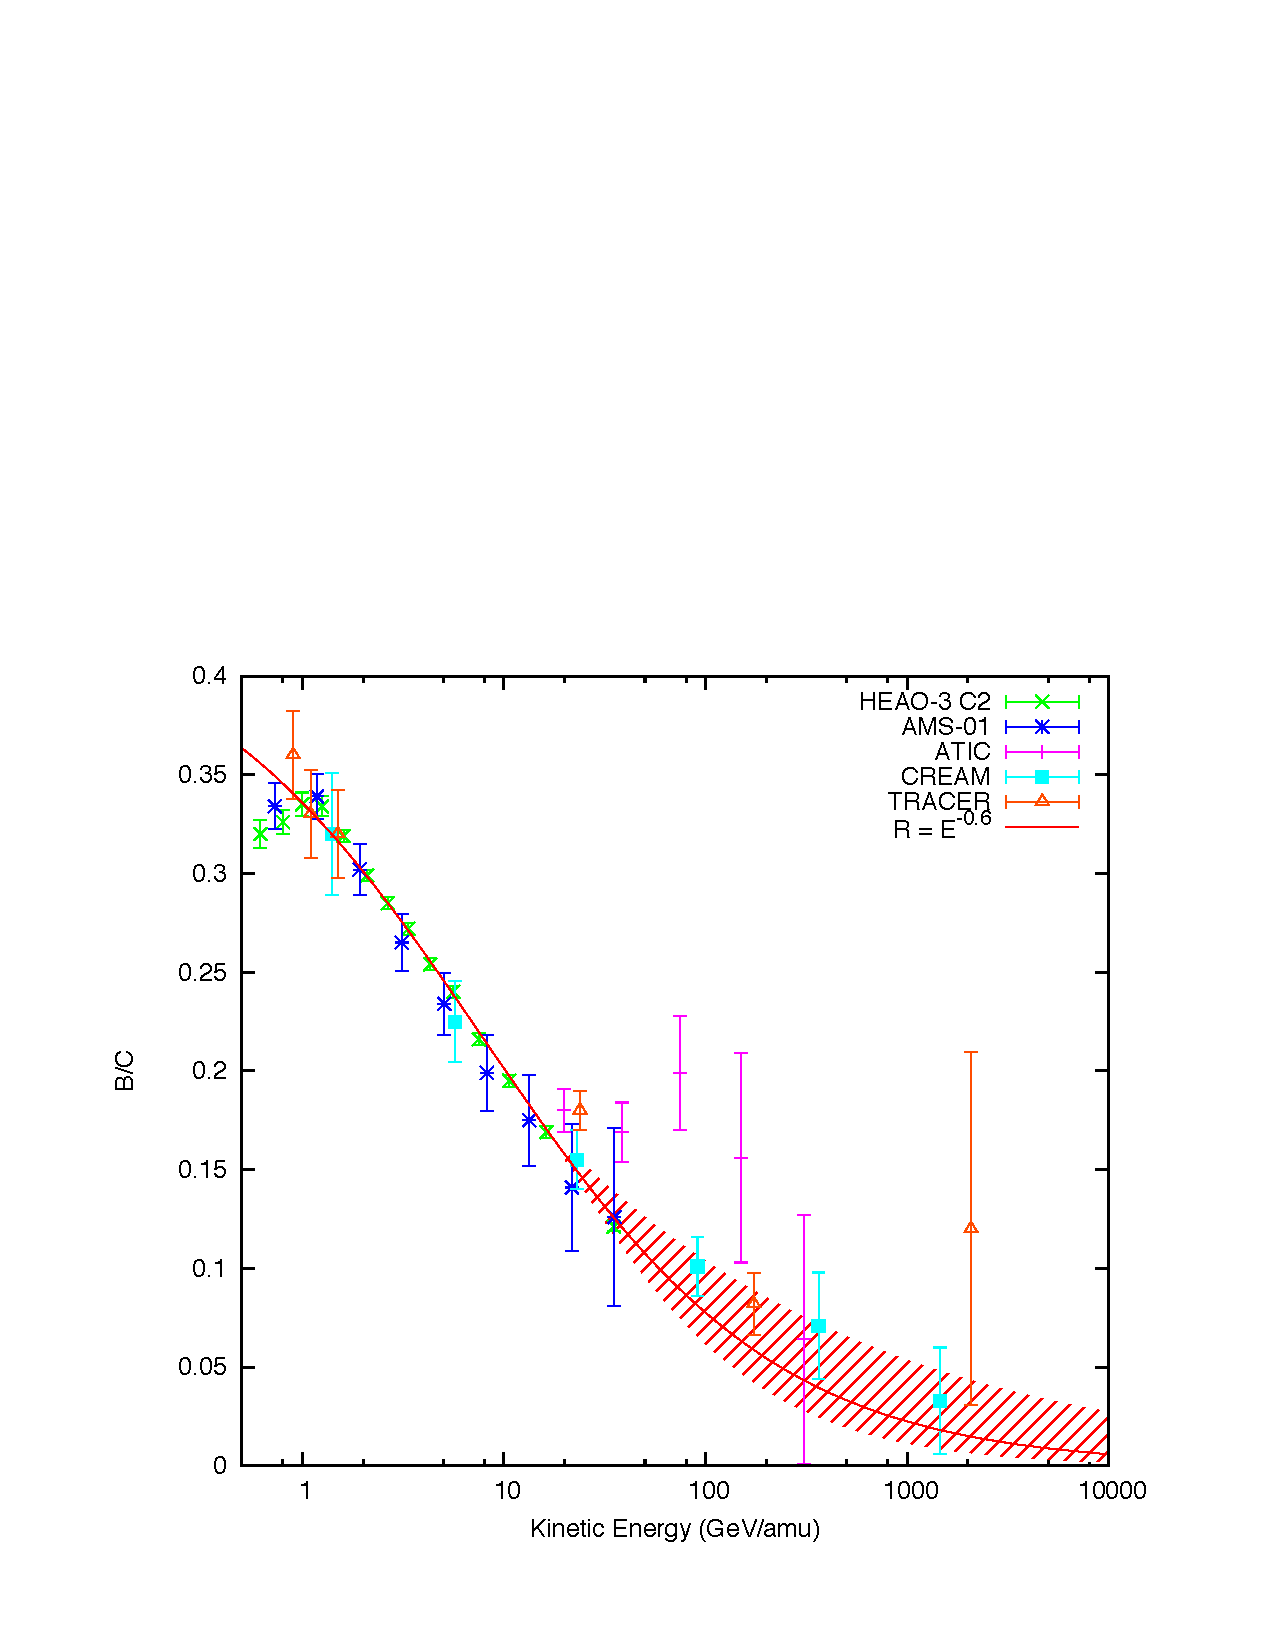
\includegraphics[width=1.08 \textwidth]{BC_ratio.pdf}
      \captionof{figure}{The Boron to Carbon ratio vs Kinetic Energy. 
  }
      
    \end{minipage}

  }


  \headerbox{The Large Area Telescope}{name=selection,column=0,span=3,
    below=goals,height=0.31}{

    \begin{minipage}[t]{0.5\textwidth}
      \vspace{0pt} % Yes: you need this one...
      
\begin{itemize}
\item The Large Area Telescope (LAT) on \emph{Fermi} is a pair conversion $\gamma$-ray telescope
\begin{itemize}
\item Field of view: 2.4 sr
\item Energy: 20MeV - 300GeV
\end{itemize}
\item The LAT has three subsystems
\begin{itemize}
\item Anti-Coincidence Detector (ACD): detects charged particles
\item Tracker (TKR): measures the direction of incoming charged particles
\item Calorimeter (CAL): measures the energy of the particle showers
\end{itemize}
\end{itemize}
\end{minipage}
\hfill
    \begin{minipage}[t]{0.45\textwidth}
      \vspace{0pt} % Yes: you need this one...      
            \centering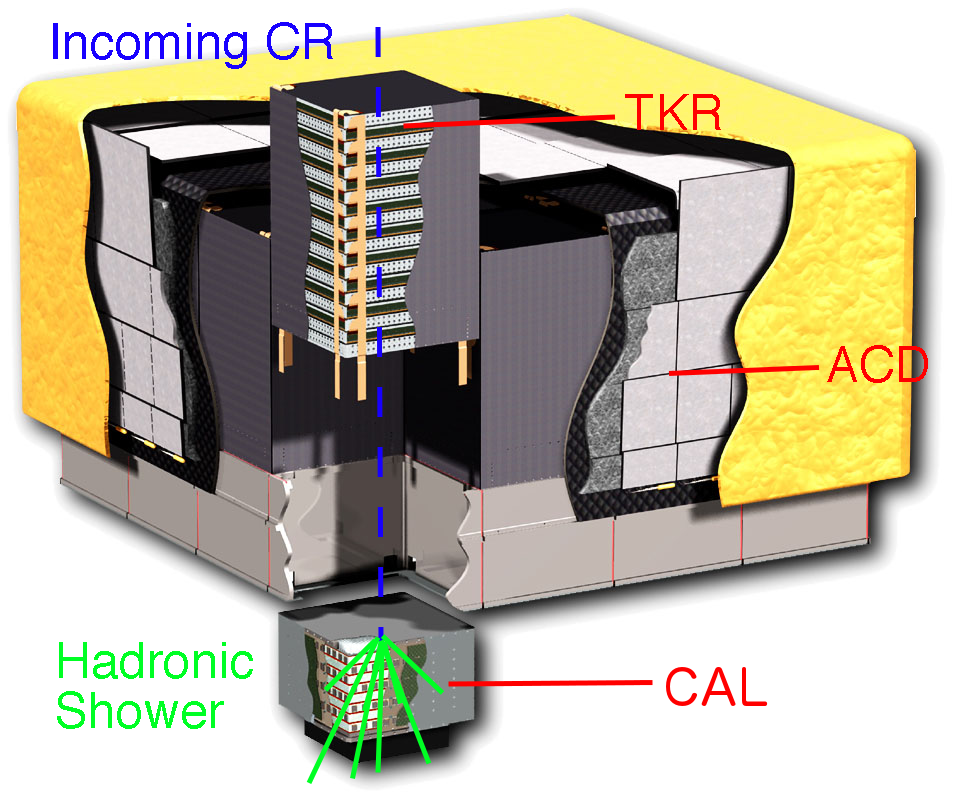
\includegraphics[width=1.08 \textwidth]{LATcutaway_full.pdf}
      \captionof{figure}{Cut a way diagram of the LAT with subsystems labeled and an example of a cosmic ray interaction.}
      
     \end{minipage}

\begin{itemize}
\item Majority of events measured by \emph{Fermi} are cosmic-rays
\begin{itemize}
\item Galactic origin energetic electrons, protons, and heavy elements (Z$\geq$3)
\end{itemize}
\item LAT is designed and calibrated for $\gamma$-ray signal 
\item We can improve LAT's ability to measure cosmic-ray nuclei
\end{itemize}

  }


  \headerbox{Selecting Cosmic-Ray Nuclei}{name=pathlength,column=0,span=3,
    below=selection,height=0.35}{

\begin{itemize}
\item Three main requirements
\begin{itemize}
\item Well reconstructed track in Tracker (TKR)
\item Large energy deposit in Anti-Coincidence Detector (ACD)
\item Energy deposit in first three layers of the Calorimeter (CAL)
\end{itemize}
\item Apply quality cuts to remove protons and poorly reconstructed events
\begin{itemize}
\item General agreement between TKR and CAL direction
\item Clean track in TKR with limited backsplash
\item Simple phenomenological model of top down hadronic shower in CAL
\end{itemize}
\item Use the better charge resolution of the CAL to initially separate cosmic-ray elements
\end{itemize}

 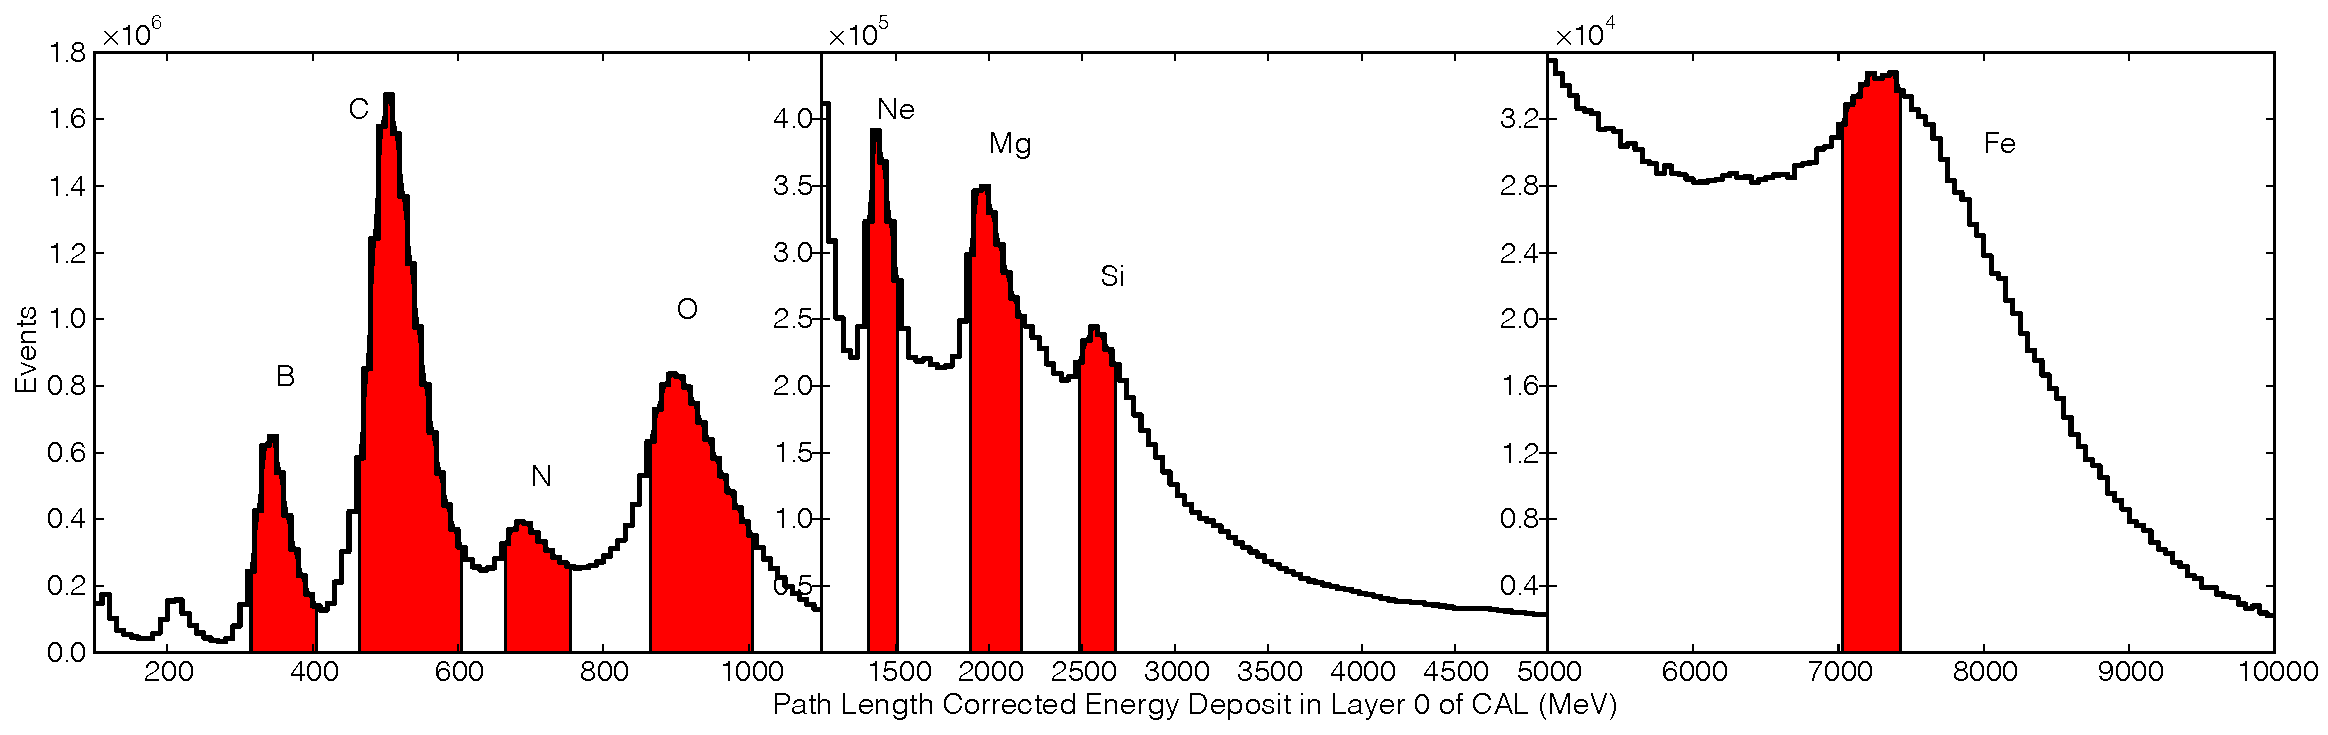
\includegraphics[width =  1.03 \textwidth]{species.pdf}  
      \captionof{figure}{Path length corrected energy deposition in the top of CAL.  Red areas indicate selection used for identification of cosmic-ray nucleus charge.}

  }


  \headerbox{Method to Improve Charge Resolution}{name=box2,column=3,span=3,
    below=abstract,height=0.215}{

    \begin{minipage}[t]{0.45\textwidth}
      \vspace{0pt} 

\begin{enumerate}
%\item Create response map for ACD signal for each element and path length through ACD
\item Average ACD signal for each element for all tiles and path length (proportional to incoming angle wrt to LAT) through ACD
%\item Determine coefficients to align each tile's element to their averages across entire ACD
%\item Plot signal for single tile vs average signal across entire ACD
%\item Fit data using power-law
\item Align each tile's signal for a given element and path length to its global average by fitting the data with a power law
\item Use coefficients from fit to determine new uniform PHA for each event
\item Apply correction coefficients and path length correction to data
\end{enumerate}


    \end{minipage}
    \hfill
    \begin{minipage}[t]{0.5\textwidth}
      \vspace{0pt} 
      \centering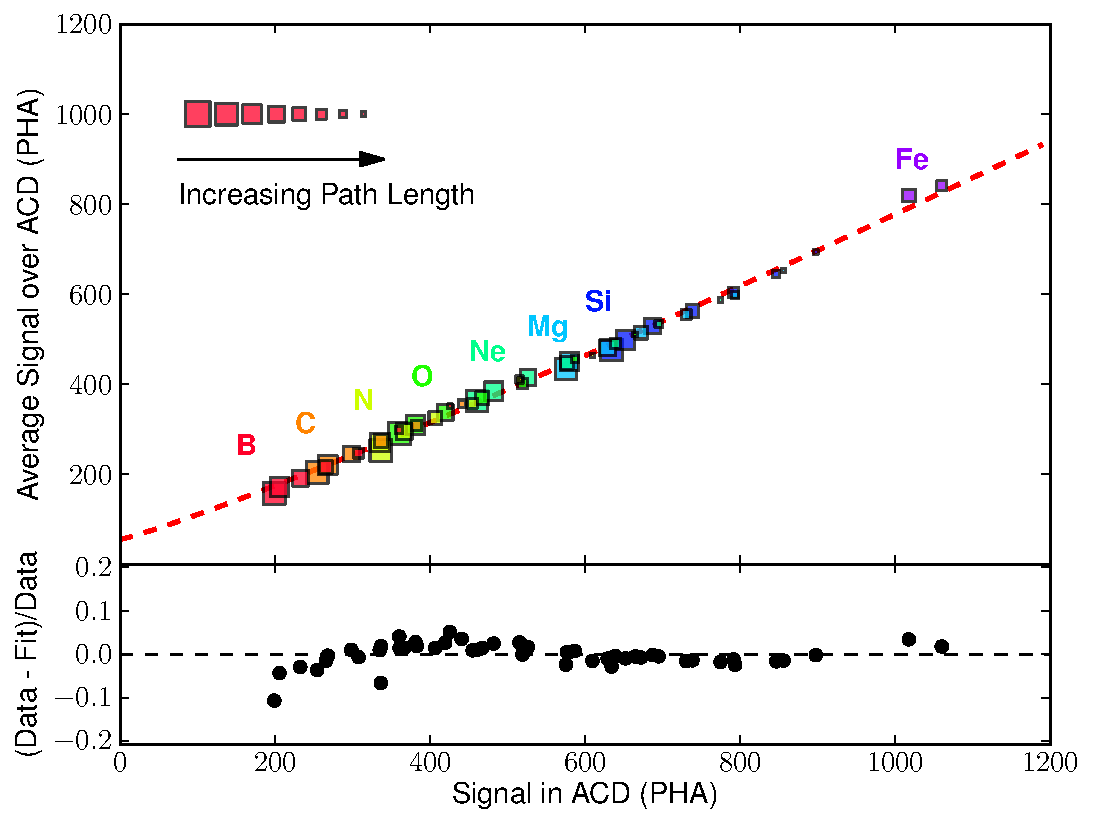
\includegraphics[width=1.07 \textwidth]{coeff.pdf}
      \captionof{figure}{Response for tile 212 PMT 0 for all charges and path lengths.}
      
    \end{minipage}
  }

  \headerbox{Charge Measurement}{name=box4,column=3,span=3,
    below=box2,height=0.235}{

    \begin{minipage}[t]{\textwidth}
      \vspace{0pt} % Yes: you need this one...

\begin{itemize}
\item B, C, O, Ne, Mg, Si and Fe peaks all become visible in ACD data
\item Uniform response improves ACD charge resolution, reduces charge overlap
\item New path length correction eliminates angular dependence in ACD data
\item Possible to use ACD (and CAL) to select cosmic ray elements
\end{itemize}

    \end{minipage}
    \hfill
%    \begin{minipage}[t]{0.5\textwidth}
%      \vspace{0pt} % ...and this one.
 %     \centering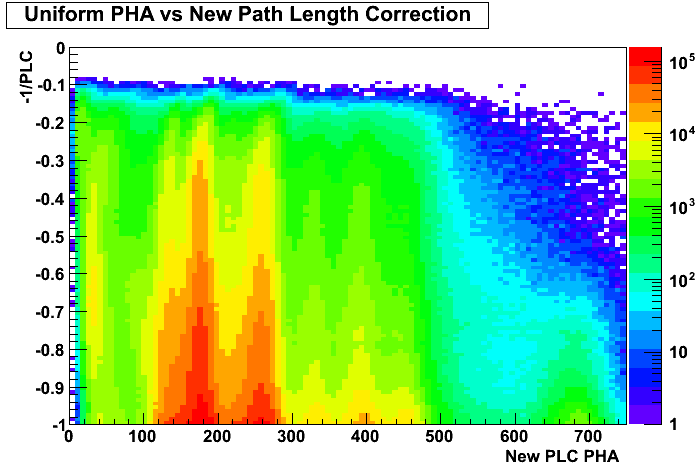
\includegraphics[width=1.05 \textwidth]{all_pLPha}
%      \captionof{figure}{Angular dependance of signal in ACD after path length correction}
      
%    \end{minipage}

      \centering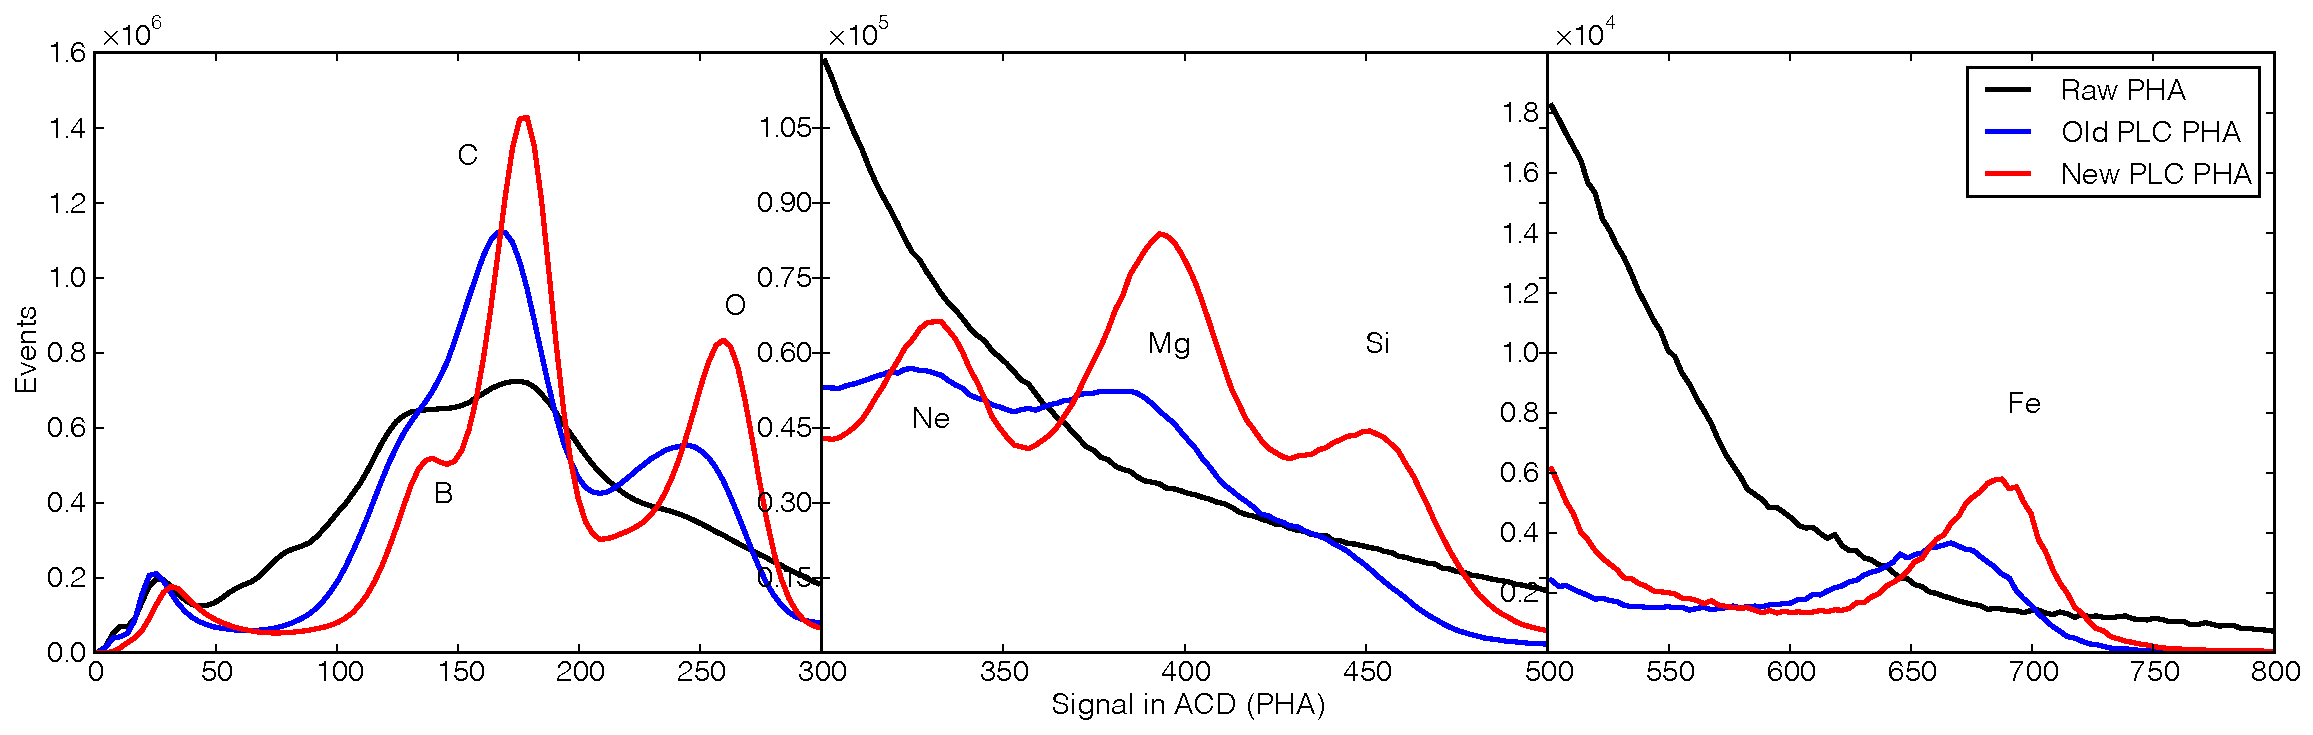
\includegraphics[width=1.03 \textwidth]{spectrum_fuck}
      \captionof{figure}{Improved charge resolution of ACD signal.}

  }



  \headerbox{Energy Measurement and the Future}{name=box5,column=3,span=3,
    below=box4,height=0.23}{
\begin{minipage}[b]{0.45 \textwidth}
      \vspace{0pt} % Yes: you need this one...
\begin{itemize}
\item Monte Carlo simulation show incident energy scales with deposited energy in CAL
\item Use long path length events to calibrate Monte Carlo simulation
\item ``Unfold" incident energy from deposited energy
\item Use charge  and energy  to measure the energy dependence of the B:C ratio
\item Explore properties of cosmic-ray propagation and the Galaxy using the B:C ratio
\end{itemize}
\end{minipage}
\hfill
\begin{minipage}[b]{0.5\textwidth}
      \vspace{0pt} % Yes: you need this one...

\centering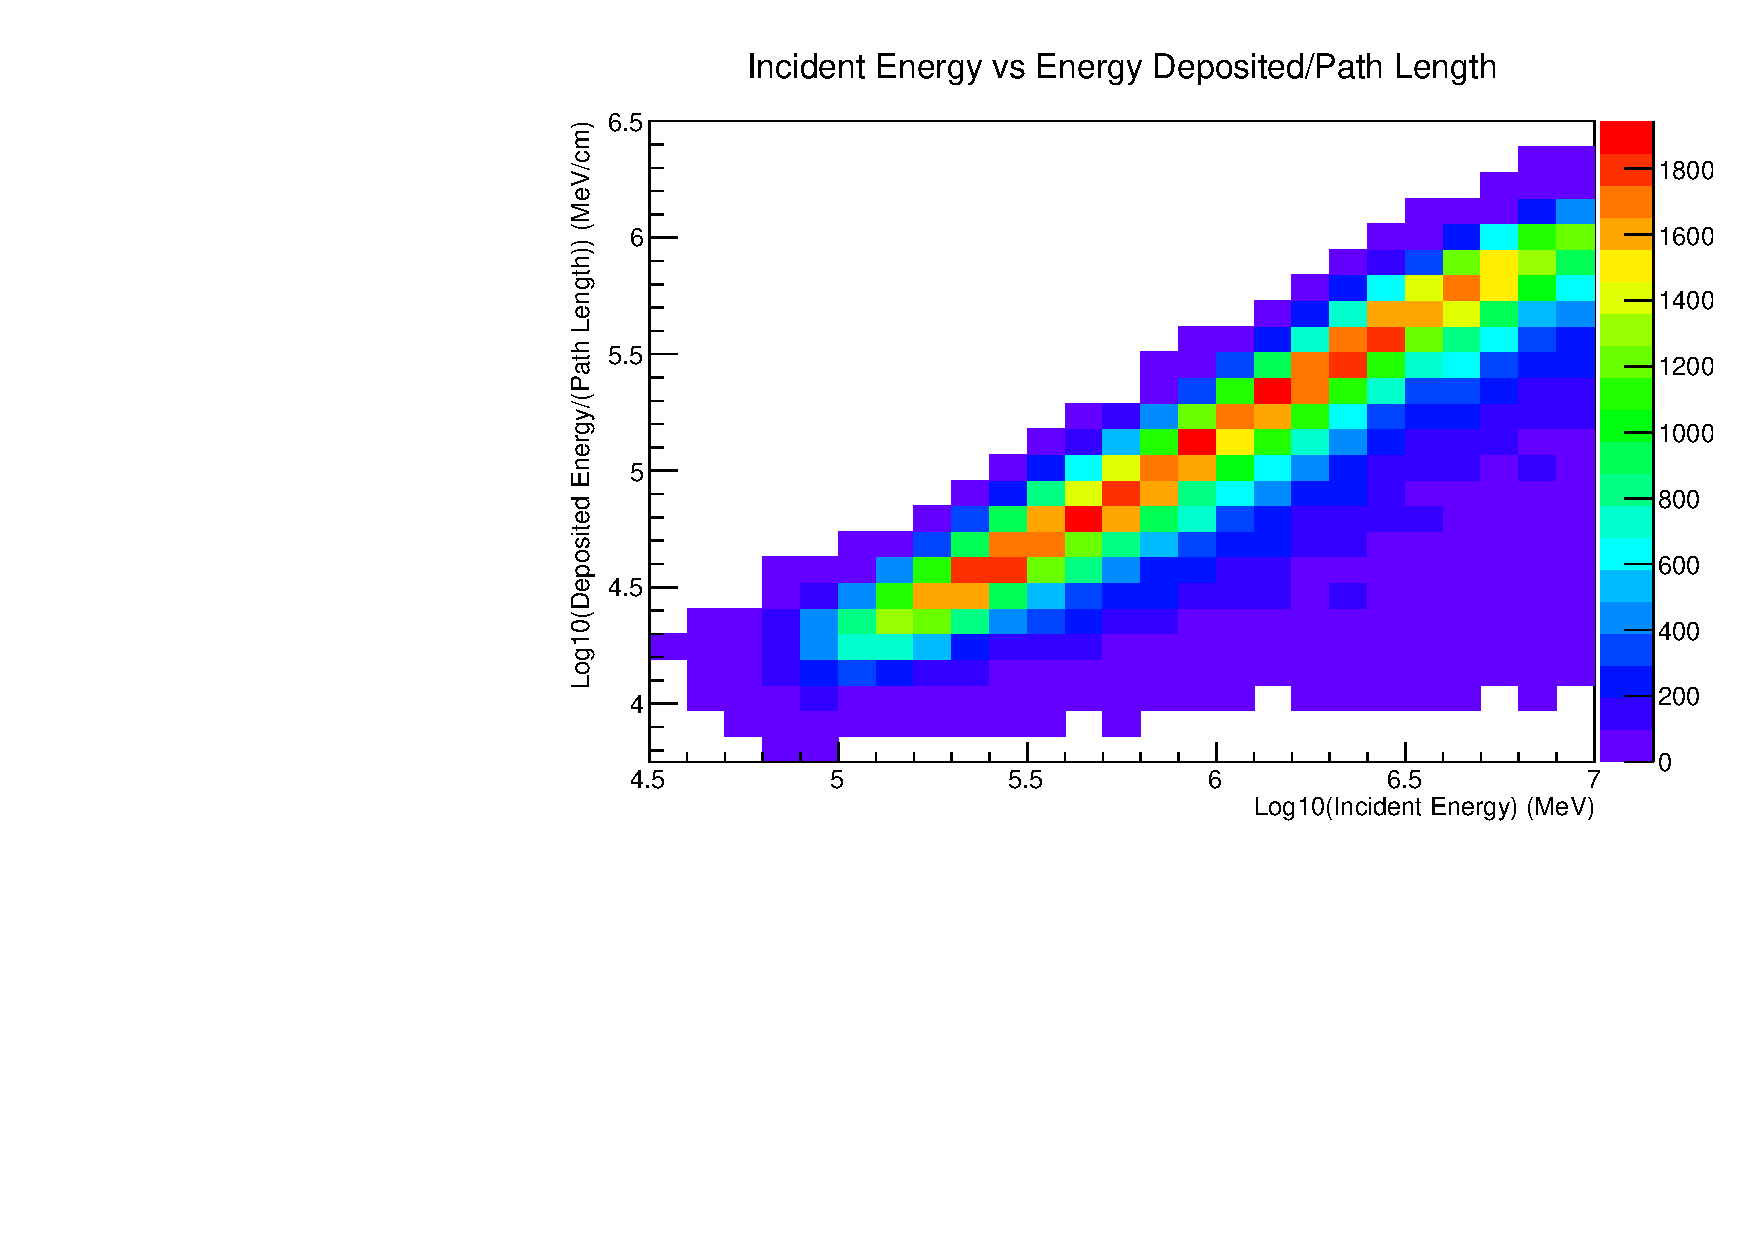
\includegraphics[width=1.08 \textwidth]{CalEnergyRaw-CalFullLen_mom12.pdf}
%\centering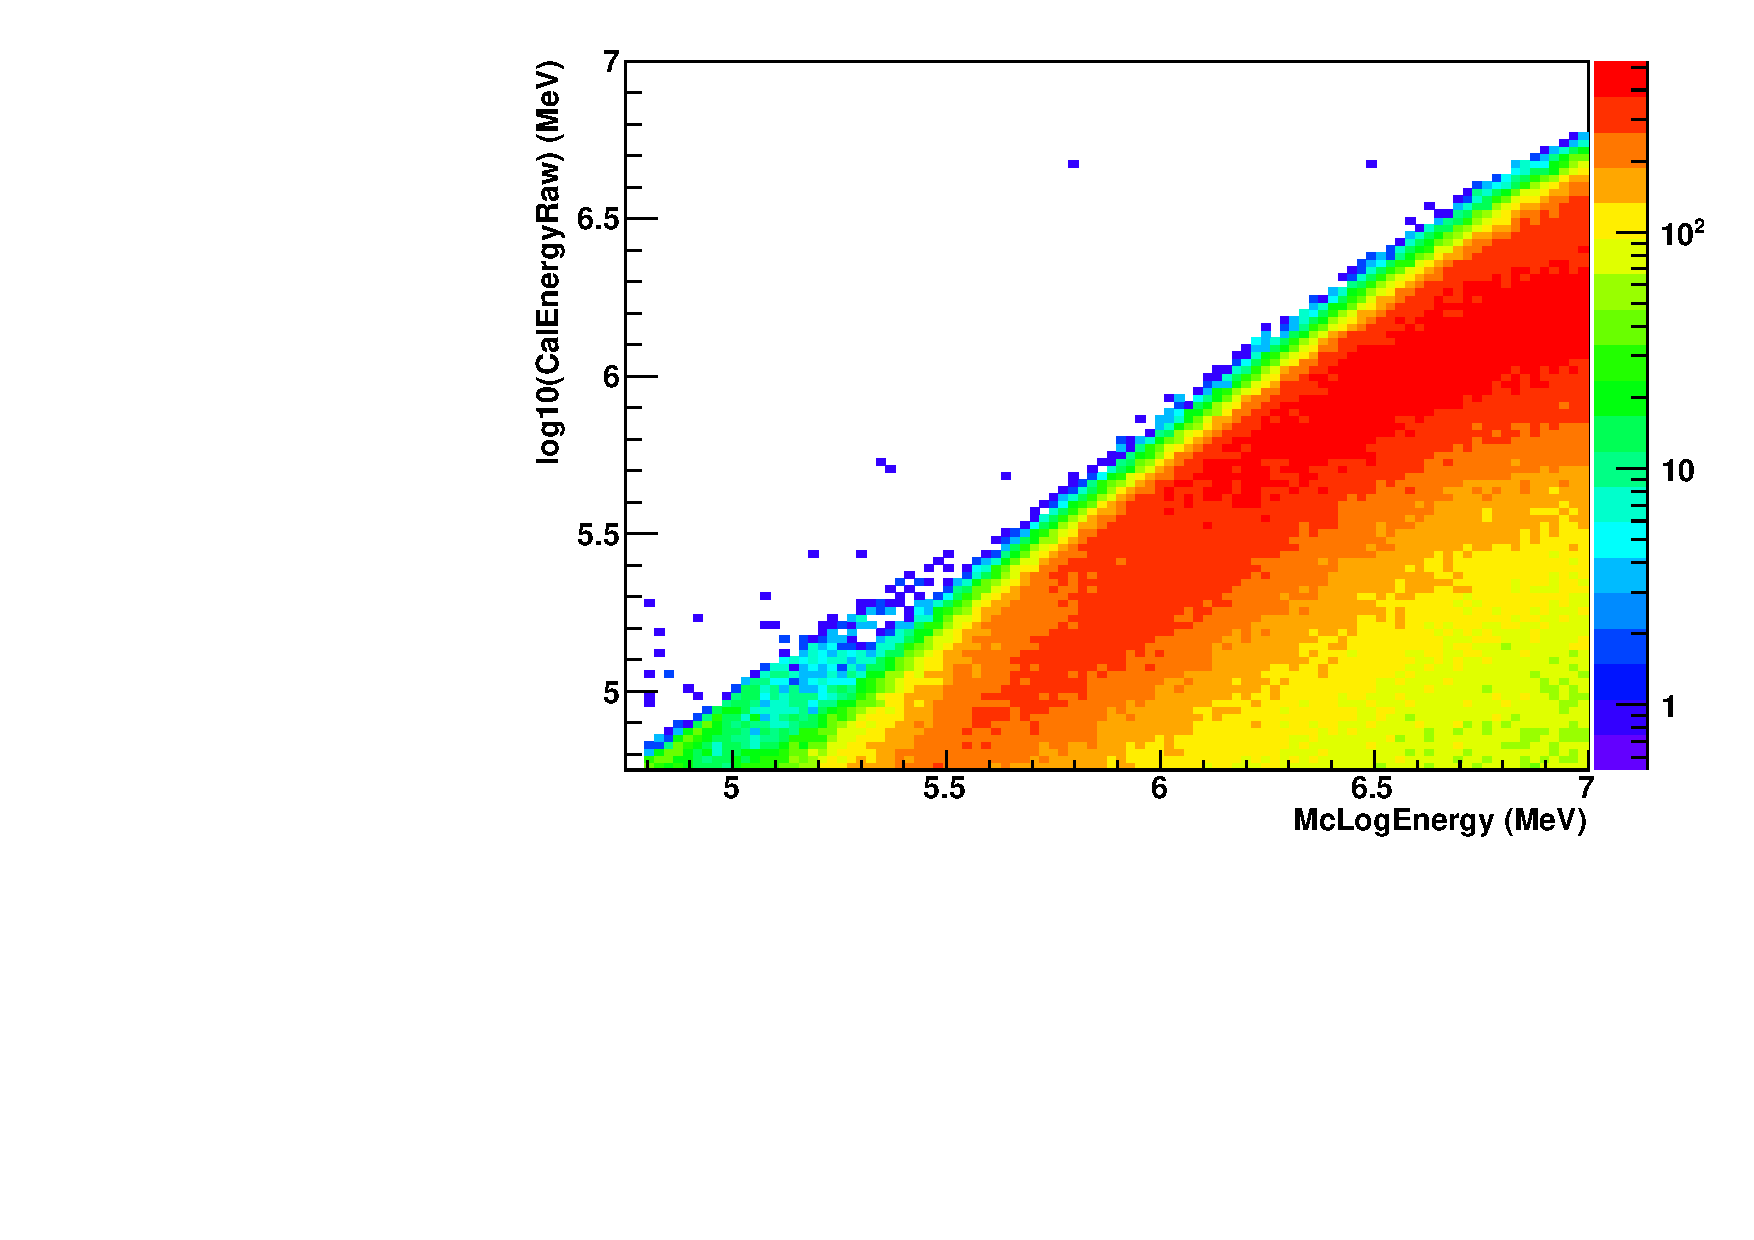
\includegraphics[width=1.08 \textwidth]{CalEnergyRaw_CalCfpEffRLn.pdf}
\captionof{figure}{Energy deposited in CAL vs Monte Carlo energy for events with $geq$ nuclear interaction length long.
% with polar angle $\theta~>~70^\circ$.
}            
\end{minipage}

}


\headerbox{Conclusion}{name=summarybox, column=3,span=3, below=box5, height=0.13}{

\begin{itemize}
\item We are able to measure cosmic-ray nuclei charge and energy with the LAT
\item ACD charge resolution is drastically improved via uniform signal and path length correction using cosmic-ray nuclei as a calibration source
\item Monte Carlo suggests correlation between energy deposited and incident energy of cosmic ray
\item Combine Z and E measurements to study the Boron to Carbon ratio
\end{itemize}
}


\headerbox{{References}}{name=ref,column=3,span=3,below=summarybox,height=0.065}{

%\item {J. J. Engelmann, P. Ferrando, A. Soutoul, P. Goret, and E. Juliusson. Charge composition and energy spectra of cosmic-ray nuclei for elements from Be to NI - Results from HEAO-3-C2. Astronomy and Astrophysics, 233(1):96-111, July 1990.}
%\item M. Aguilar et. al. Relative Composition and Energy Spectra of Light Nuclei in Cosmic Rays: Results from AMS-01. The Astrophysical Journal, 724(1):329, 2010.
%\item A. D. Panov et. al. Relative abundances of cosmic ray nuclei B-C-N-O in the energy region from 10 GeV/n to 300 GeV/n. Results from ATIC-2 (the science flight of ATIC). In Rogelio Caballero, Juan Carlos D�Olivo, Gustavo Medina-Tanco, Lukas Nellen, Federico A. S?anchez, and Jos?e F. Vald?es-Galicia, editors, Proceedings of the 30th International Cosmic Ray Conference, volume 2, pages 3-6. Universidad Nacional Aut?onoma de M?exico, 2008.
%\item H.S. Ahn et. al. Measurements of cosmic-ray secondary nuclei at high energies with the first flight of the CREAM balloon-borne experiment. Astroparticle Physics, 30(3):133 - 141, 2008.
%\item A. Obermeier, M. Ave, P. Boyle, Ch. H?oppner, J. H?orandel, and D. Mu?ller. Energy spectra of primary and secondary cosmic-ray nuclei measured with TRACER. Astrophysical Journal, 742:14, 2011.

%\item HEAO-3-C2. A\&A, 233(1):96-111, July 1990.
%\item AMS-01. ApJ, 724(1):329, 2010.
%\item ATIC-2. ICRC 30th. Vol 2:3-6, 2008.
%\item CREAM. AP, 30(3):133 - 141, 2008.
%\item TRACER. ApJ, 742:14, 2011.


    \begin{minipage}[t]{0.45\textwidth}
      \vspace{0pt} % Yes: you need this one...
\tiny{
\begin{enumerate}
\item HEAO-3-C2. A\&A, 233(1):96-111, July 1990.
\item AMS-01. ApJ, 724(1):329, 2010.
%\item AMS-02. ICRC 33th.  To be published.
\item ATIC-2. ICRC 30th. Vol 2:3-6, 2008.
\end{enumerate}
}
    \end{minipage}
    \hfill
    \begin{minipage}[t]{0.5\textwidth}
      \vspace{0pt} % ...and this one.
 \tiny{ 
\begin{enumerate}
\setcounter{enumi}{3}
\item CREAM. A Phys, 30(3):133 - 141, 2008.
\item TRACER. ApJ, 742:14, 2011.
\item ACD. A Phys, 27:339-358, February 2007.
\end{enumerate}      }
    \end{minipage}

}

\end{poster}

\end{document}
